\documentclass[output=paper]{LSP/langsci}  
\author{Takuichiro Onishi\affiliation{National Institute for Japanese Language and Linguistics}} 
\title{Timespan comparison of dialectal distributions}
\abstract{Traditional Japanese dialectology has held that dialectal distributions are caused by the diffusion of language changes from a central area, as in the dialect radiation theory. If this is true, then we can capture the radial spread of changes in dialectal distributions by surveying an area over a period of time. Since Japanese dialectology has published many dialect maps, we have at least half a century’s excellent geolinguistic data. We have researched the same area with the same methodology of past geolinguistic surveys to compare the dialectal distributions over a timespan of 30 to 50 years. This study shows two main results. The first is that changes in dialectal distributions are neither continual nor gradual. Diffusions are completed in one breath, and the new forms cover each area quickly. The second result is that dialectal distributions do not change easily. Many features have retained their past distributions. These results inform our knowledge of language change and dialect formation. Dialect is a means for people to communicate with one other; once a language change occurs, the change should spread throughout the community to maintain communication. Language change is the unpreferred option, since linguistic variation introduced by language change can impede smooth communication.
}

\maketitle 
\begin{document}
 
 
% 
% \vskip11pt
% \\
% 
 
\section{Introduction}

How do time and space relate in dialects, especially in dialectal distributions? According to traditional Japanese dialectology, dialectal distributions are caused by the diffusion of linguistic changes from a central area to surrounding areas. This idea has been known as the dialect radiation theory since \citet{yanagita_kagyuukoo._1930}. If this is correct, we should be able to capture radial changes in dialectal distributions when we survey an area over a period of, for example, 30 to 50 years.

Since Japanese dialectologists have published over 400 dialectal atlases over the last 50 years, including 30,000 maps of dialectal distributions, we have at least half a century’s excellent geolinguistic data both for Japan as a whole and for specific regions. We have investigated the same areas with the same methods as in past geolinguistic surveys to compare the distributions we find over the timespan of 30 to 50 years with the distributions predicted by traditional Japanese dialectology.

We have reached two main results in this study. The first result is that changes of dialectal distributions are neither continual nor gradual. The pattern of diffusion seems not to be expansion but rather filling. The diffusions we studied were completed in one breath, and the new forms covered each area quickly. The second result is that dialectal distributions do not change often. We expected that more changes of dialectal distributions would easily be captured through the investigation, since traditional Japanese geolinguistics interprets dialectal distributions as expanding diffusions of continual linguistic changes from the center. However, many of the distributions have kept their past conditions.

These results suggest that linguistic changes and spatial formations (including geographical boundaries) of dialects are related. The purpose of dialect, and indeed that of any language variety, is communication; once a linguistic change has occurred, it should diffuse quickly to support communication. On the other hand, it is better for a language not to change, since variation caused by linguistic change can block smooth communication. Therefore, after finishing a linguistic change, dialectal distributions become stable once again.

The examples presented in this paper include that of  a grammatical item in a large area and those of lexical items in a smaller area. 

\section{Real-time research on dialectal distributions}

We are conducting three projects comparing modern dialectal distributions to past dialectal distributions. Within each project, data has been acquired over a 30- to 50-year period. One project treats a wide area (all of Japan),  the others treat smaller areas (separate regions). The informants in each project were around 70 years old at the time of the investigation.

The projects use data from three linguistic surveys. The Field Research Project to Analyze the Formation Process of Japanese Dialects (FPJD) has conducted research in 500 places across Japan between 2010 and 2014. The Linguistic Atlas of Japan (LAJ) project mainly investigated lexical items in 2,400 places around 50 years ago (1957--1965). The Grammar Atlas of Japanese Dialects (GAJ) project investigated grammatical items in 800 locations about 30 years ago (1979--1982). In this paper, I compare data from FPJD to data from GAJ, a real-time interval of 30 years.

In collaboration with Professor Seiichi Nakai of Toyama University, I investigated around 200 locations in the Shogawa River basin in Toyama prefecture between 2009 and 2012, and compared the results to the data from \citet{sanada_ecchu-hida_1976}. \citeauthor{sanada_ecchu-hida_1976} investigated the upper regions of Shogawa River basin between 1967 and 1969. The timespan between Sanada’s and the present study is 40 years.

In an ongoing collaboration with Professor Motoei Sawaki of Shinshuu University, we investigated some 200 locations in the Ina and Suwa regions in Nagano prefecture between 2010 and 2013 for a comparison with the data from \citet{mase_kami-ina-no_1980}. \citeauthor{mase_kami-ina-no_1980} investigated this area between 1968 and 1973, so real-time data is available for a 40-year interval.

\section{Language change and dialectal distributions}\label{sec:lgchdialdist}
In this section, I present my hypothesis of how linguistic changes proceed in dialectal distributions, and I suggest a concrete verification.

In the event of a linguistic change, dialectal distributions are expected to change as in \figref{fig:1}. Initially, features x and y are distributed as in the left-hand panel (a). The feature x changes to z in some locations; as a result, the dialectal distribution changes as indicated in the right-hand panel (b).

\begin{figure}
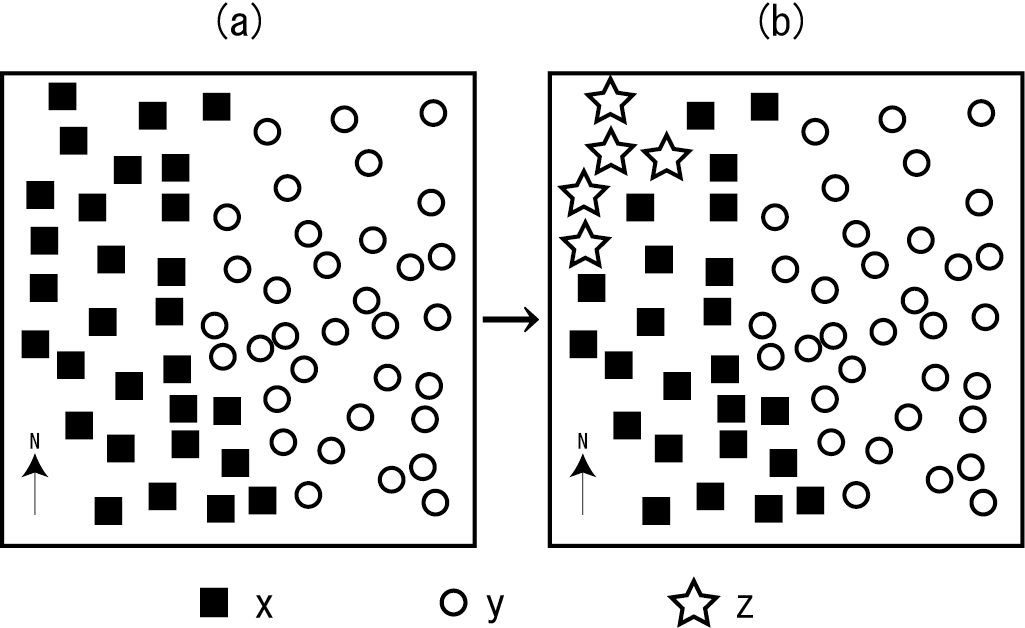
\includegraphics[width=\textwidth]{illustrations/onishi_fig1}
\caption{Linguistic change and change in dialectal distributions.}
\label{fig:1}
\end{figure}

Evidence comes from change in the past-tense negative verb suffix. The form \textit{-nanda} was the standard form and was used in official written language in the early modern period; for example, \textit{nom-u} ‘drink’, \textit{nom-a=N}\footnote{ The present-tense negative suffix of verbs \textit{-n} is written \textit{-N} in this paper as it is pronounced as one syllable. The present-tense negative suffix is a well-known feature dividing Japanese dialects into east and west: \textit{-N} is used in the western area and \textit{-nai} in the eastern area. \textit{-nai} is the standard Japanese form, since the capital city Tokyo is in the eastern area.} ‘do not drink’, \textit{nom-a=nanda} ‘did not drink’. However, \textit{{}-nanda} is not a well-segmented form. It is not clear which segment in \textit{-nanda} expresses negation, and the form has an unclear etymology \citep{onishi_atarashii_1999}. In terms of grammar, verbs are dynamic (+activity, -condition), but negative verbs become static (or stative) (-activity, +condition) and similar to adjectives, which are also static rather than dynamic. \textit{-Nkatta} is a newly occurring form of the past-tense negative verb suffix in some dialects, the final element \textit{{}-katta} coming from the past-tense form of adjectives; for example, \textit{taka-i} ‘be high’, \textit{taka-katta} ‘was high’,  so also \textit{nom-a=N} ‘do not drink’, \textit{nom-a=Nkatta} ‘did not drink’. \textit{-Nkatta} is a dialectal form and is used in spoken but not written language. Modern standard Japanese uses \textit{–nakatta}, which is different from the dialectal form \textit{-Nkatta}. 

\figref{fig:2} shows that \textit{-nanda} was used almost everywhere in Osaka\footnote{ The Osaka dialect is representative of western dialects of Japanese; Osaka prefecture is a core area in  western Japan with a population of 8 million.} in the GAJ data from around 1980. Few places in the area used \textit{{}-Nkatta} as the past-tense negative verb suffix. \citet{sanada_kansaihougen-no_1992} reported a change from \textit{-nanda} to \textit{-Nkatta} in Osaka\footnote{ \citeauthor{sanada_kansaihougen-no_1992}'s (\citeyear{sanada_kansaihougen-no_1992}) interpretation of the change is that \textit{-Nkatta} was formed under the influence of standard Japanese \textit{-nakatta}.}. \citeauthor{sanada_kansaihougen-no_1992}'s data is shown in  \figref{fig:3}. Speaker age in this graph is at the time of investigation (1988--1989); the informants in FPJD correspond to the 50-year-old age group in \citet{sanada_kansaihougen-no_1992}. The FPJD data (\figref{fig:4}) clearly shows an expanded distribution for \textit{-Nkatta}. When we compare \figref{fig:2} and \figref{fig:4}, we see that part of the area of distribution for \textit{-nanda} shows a change to \textit{-Nkatta}, similar to the model presented in \figref{fig:1}. This example verifies the hypothesis of the link between language change and a change in dialectal distribution.


\begin{figure}
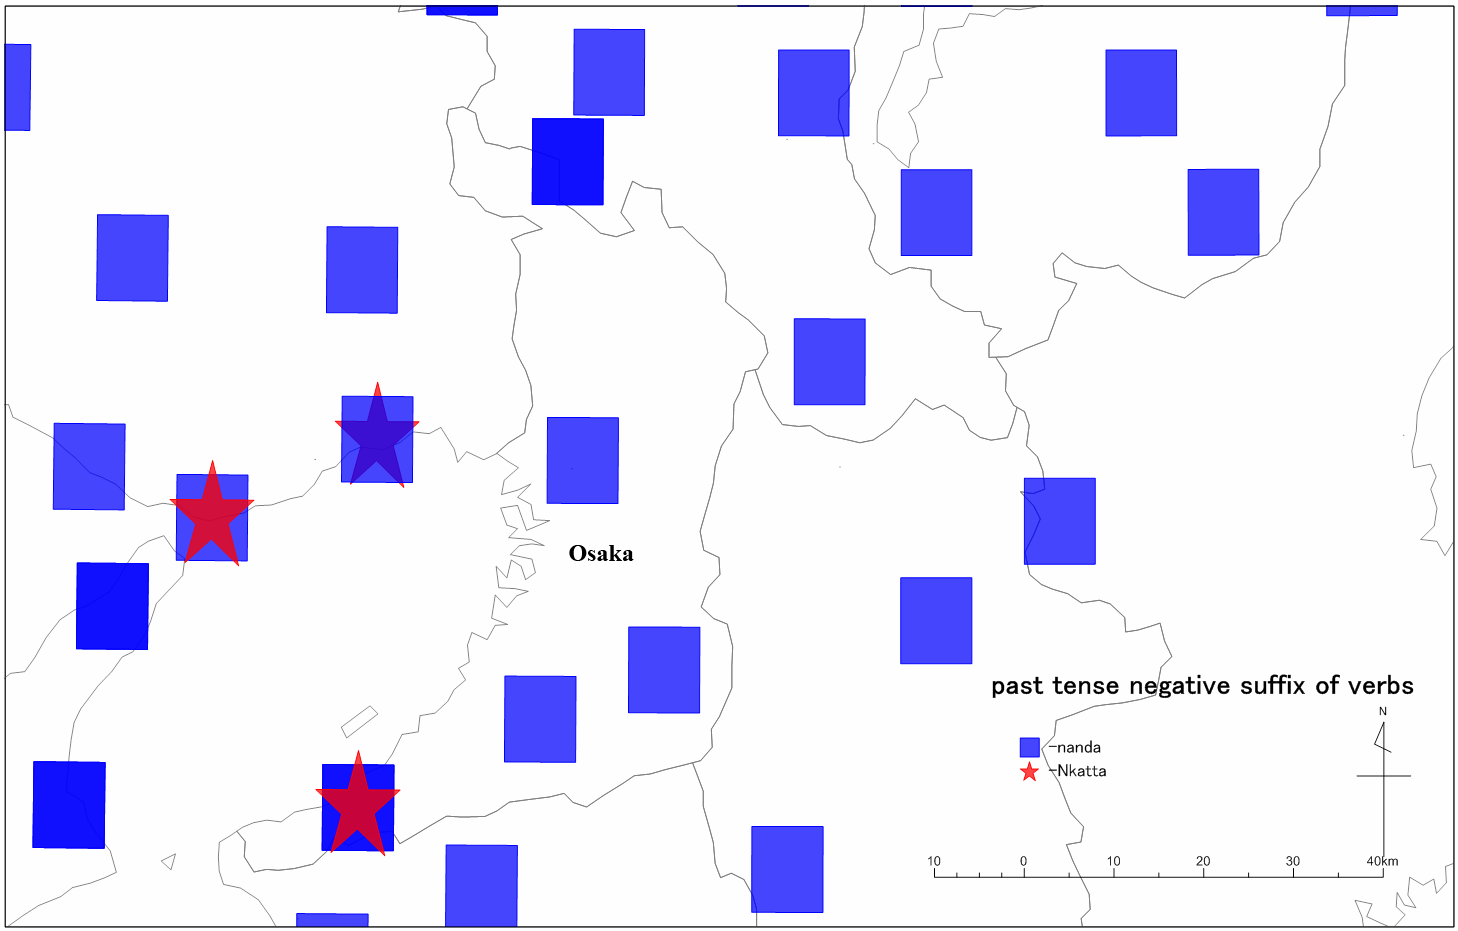
\includegraphics[width=\textwidth]{illustrations/onishi_fig2}
\caption{Dialectal distributions of the past-tense negative verb suffixes in Osaka in the GAJ (around 1980).}
\label{fig:2}
\end{figure}

 
\begin{figure}
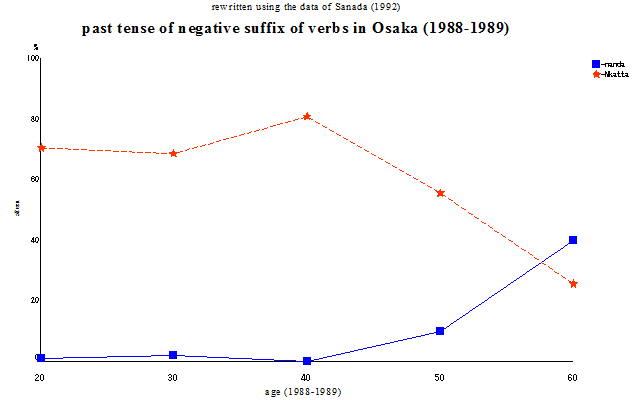
\includegraphics[width=\textwidth]{illustrations/onishi_fig3}
\caption{Linguistic change of \textit{-nanda} to \textit{-Nkatta} in Osaka. Based on data from \citet{sanada_kansaihougen-no_1992}.}
\label{fig:3}
\end{figure}

\begin{figure}
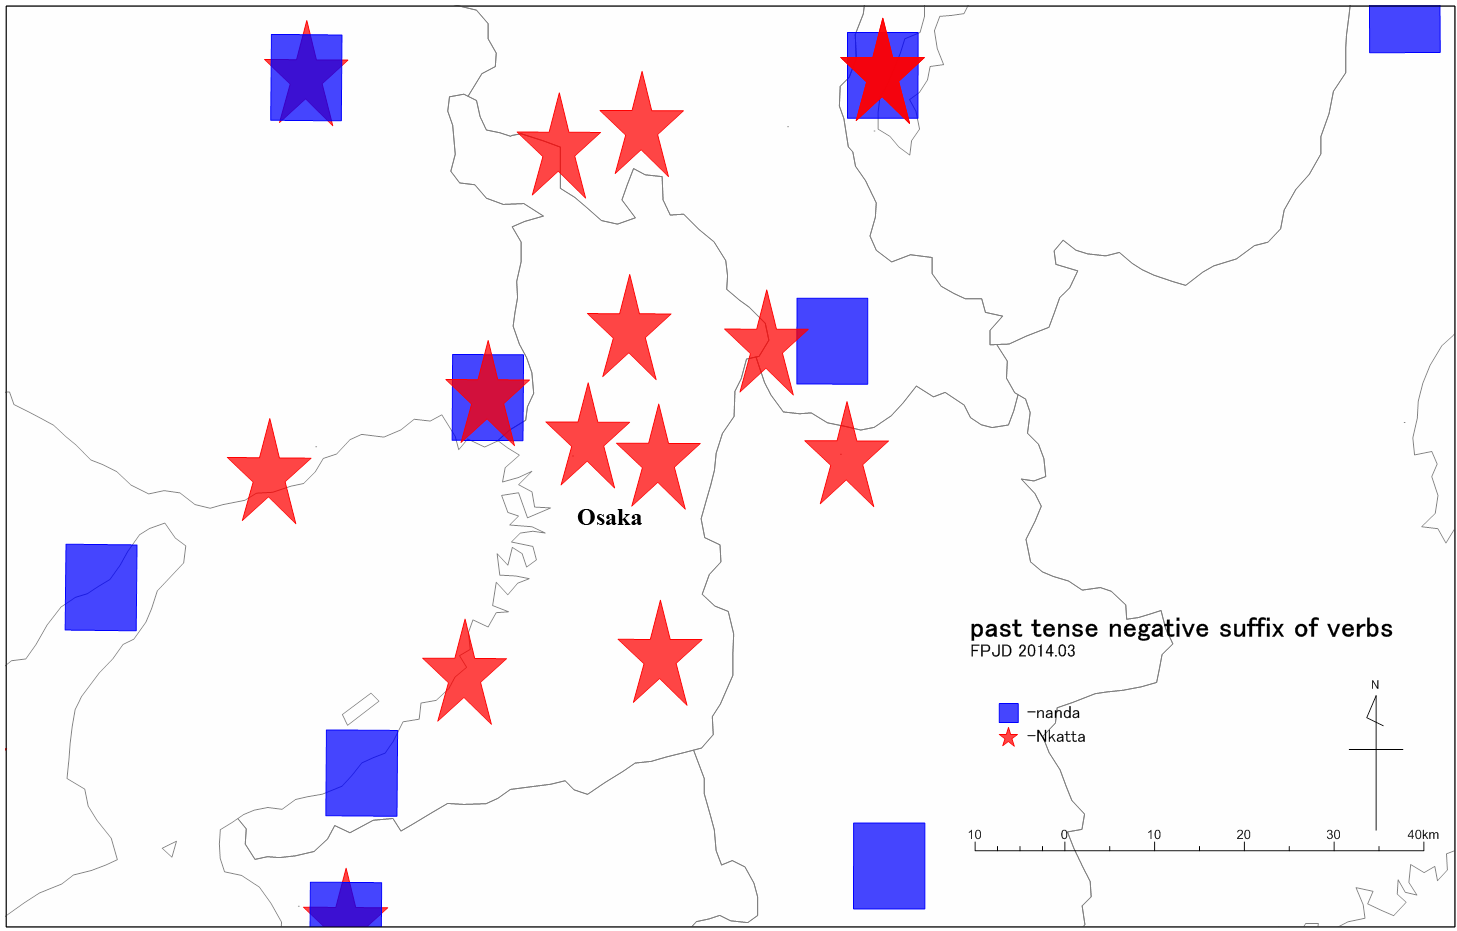
\includegraphics[width=\textwidth]{illustrations/onishi_fig4}
\caption{Dialectal distributions of past-tense negative verb suffixes in Osaka according in FPJD (around 2010).}
\label{fig:4}
\end{figure}

\section{Real-time comparison of dialectal distributions}
A comparison of other maps of dialectal distributions shows that changes in dialectal distributions are quick rather than gradual; in some cases, the distributions do not change at all.

\subsection{Rapid change}
Since our comparison of real-time data of dialectal distributions is limited to two generations, it is difficult to see the precise stages in which change has occurred. However, when changes do occur, they seem to spread through the area in 30 to 50 years, which is more rapid than we expected.

\figref{fig:5} shows the change in distribution of \textsc{bebe}\footnote{ Small capitals denote umbrella terms for some of the variants in \figref{fig:5} and \figref{fig:7}.} forms of the name for the tick-trefoil plant in the Chino area in the Ina-Suwa region.\footnote{ The dialect in this area is representative of Tokai-Tosan dialects and is classified as an eastern Japanese dialect.} The \textit{bebe-} in \textit{bebebasami} and \textit{bebekkusa} is related to the word for `clothes'; \textit{basami} is `putting', and \textit{kusa} is `grasses'. The names come from the nature of this plant: seeds of the plant stick to the clothes of those walking in the fields or mountains.

\textsc{bebe} forms were used in the Chino area 40 years ago, as the blue symbols in \figref{fig:5} show. In the FPJD data, 40 years later, new words occur: \textit{zizibasami} and \textit{chinkorobasami}.  \textit{Zizi-} is related to the word for `old man, grandfather' and occurs under folk etymology and paronymic attraction to \textit{baba} `old woman, grandmother', cf.\ the original form \textit{bebe}. \textit{Chinkoro-} refers to the male genital organ, and is associated in folk etymology to a homonym of \textit{bebe} `female genital organ'.

\textit{Zizibasami} appears to have diffused in the area of high elevation, and \textit{chinkorobasami} in areas of mid-high elevation. People at the same elevation in these two areas are said to form communities; for example, they have traditionally established marital relations within the contour lines depicting elevation on maps of the area. The diffusing areas of new words for the tick-trefoil plant match these small community areas.

As shown in Section \ref{sec:lgchdialdist}, the area of distribution of the past-tense negative verb suffix \textit{-Nkatta} formed rapidly in Osaka. The same change is seen in Aichi, on the border between eastern and western dialect areas of Japanese. The GAJ data (\figref{fig:6}) shows that \textit{-Nkatta} was used in a small part of the Aichi area 30 years ago, but since then it has spread to the entire area.

In these cases of language change -- the past-tense negative verb suffix in Osaka and Aichi, and the name of the tick-trefoil plant in Chino -- the new forms seem to diffuse as if to fill the community areas, i.e., the prefecture areas of Osaka and Aichi, and areas with the same elevation in Chino. Diffusion of features does not happen in a radiating pattern from the center, since the new forms \textit{-Nkatta}, \textit{zizibasami} and \textit{chinkorobasami} originate in the area surrounding Osaka rather than in Osaka itself (\figref{fig:2}), in the rural area of Aichi rather than in its capital city Nagoya (\figref{fig:6}),\footnote{ Nagoya is the largest city in this area with a population of approx.\ 2 million.} and in the more elevated agricultural area in Chino (\figref{fig:5}).


\begin{figure}
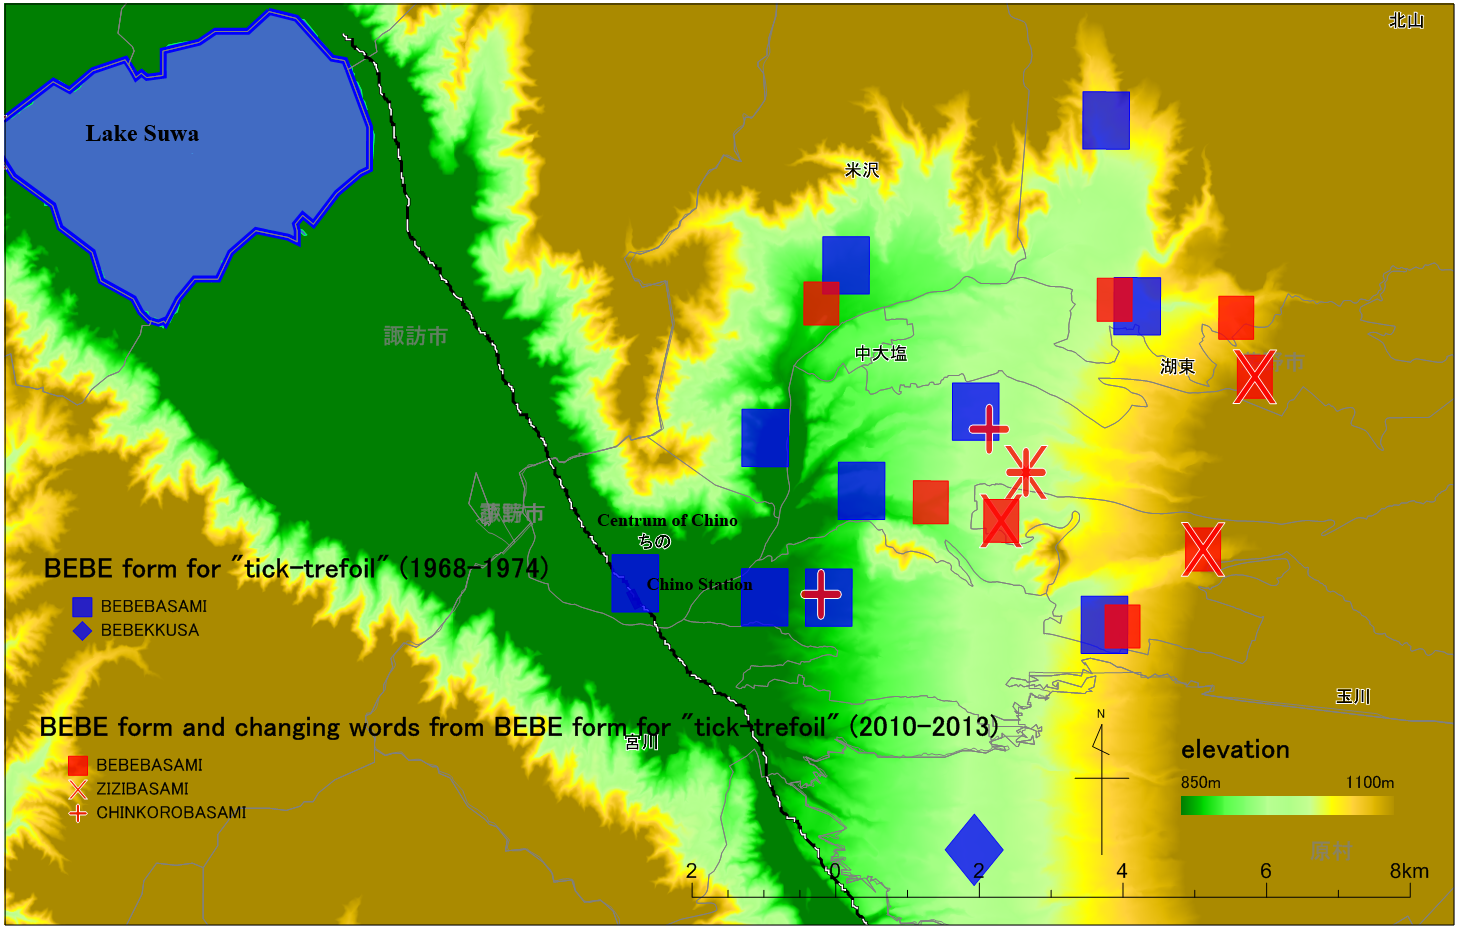
\includegraphics[width=\textwidth]{illustrations/onishi_fig5}
\caption{The distribution of \textsc{bebe} forms and the spread of alternative names for the tick-trefoil plant in the Chino area in the Ina-Suwa region.}
\label{fig:5}
\end{figure}

\begin{figure}
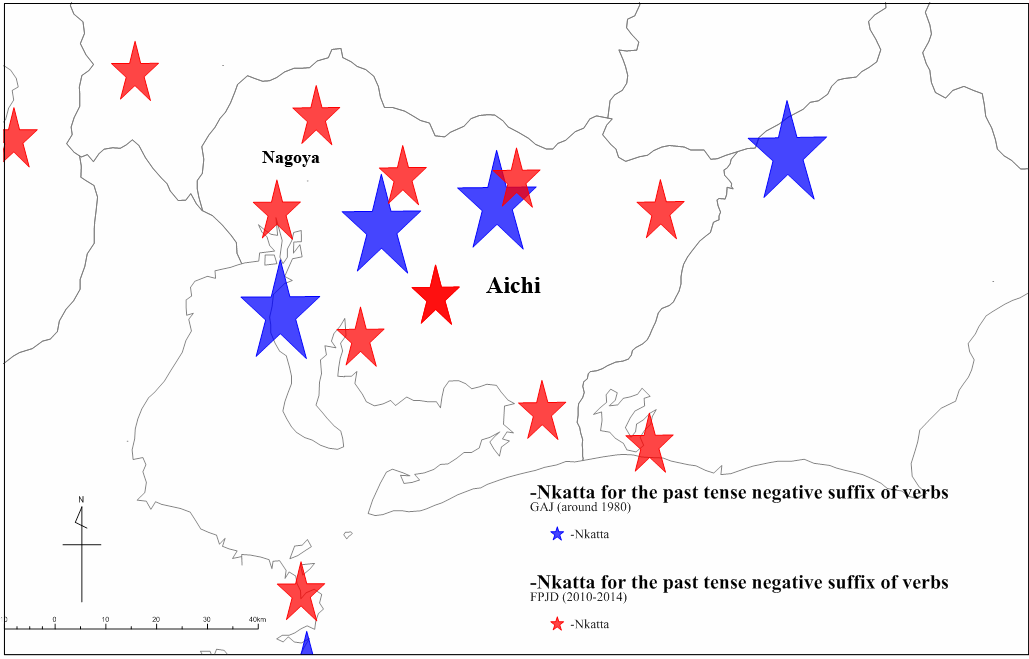
\includegraphics[width=\textwidth]{illustrations/onishi_fig6}
\caption{The spread of the past-tense negative suffix \textit{-Nkatta} over a 30-year period in the Aichi region.}
\label{fig:6}
\end{figure}

\subsection{Standstills}
\figref{fig:7} shows the distribution of names for a fruit-like potato, growing from the branches of Japanese yam roots (Standard Japanese \textit{mukago}) in the Shogawa River basin.\footnote{ The Shogawa River flows from south to north. The southern, upper reaches form an agricultural area; the northern, lower reaches are an urban area.} The map overlays data from 40 years ago with the current distribution of names.

\begin{figure}
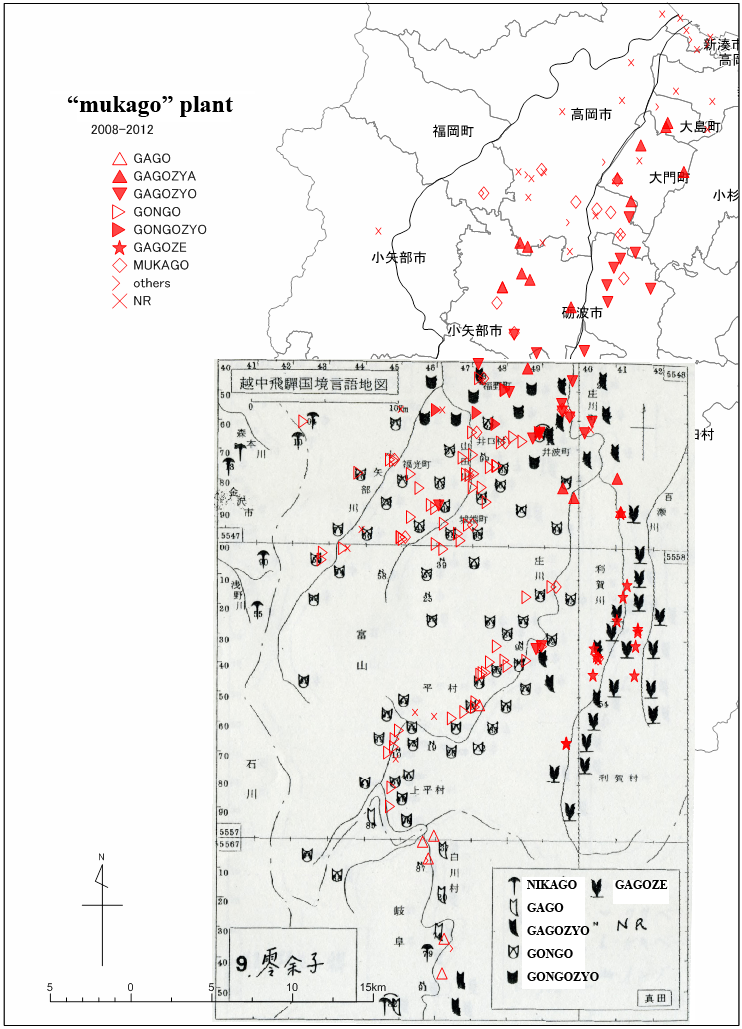
\includegraphics[width=\textwidth]{illustrations/onishi_fig7}
\caption{Distribution of names for the \textit{mukago} plant in the Shogawa River basin over a 40-year period. The older map, in black and white, is taken from \citet{sanada_ecchu-hida_1976}.}
\label{fig:7}
\end{figure}

In the older data, words ending in \textsc{-zyo} (\textit{gagozyo}, \textit{gongozyo}) were found in lower areas in the north, whereas words without \textsc{-zyo} (\textit{gago}, \textit{gongo}) were found in higher areas in the south. Comparing this data to the present-day distribution, we make two important observations. Firstly, the basic distribution has been maintained, with lower regions using the \textsc{-zyo} ending and higher regions using forms without \textsc{-zyo}. The isogloss has not changed significantly. Secondly, within this stable pattern, more detailed distributions have been maintained. For instance, in the southern, higher area, a word with \textsc{-zyo} exists on the east bank of the river. These results indicate that the dialectal distribution of names for the \textit{mukago} plant has not changed in the last 40 years \citep{onishi_relationship_inprint}.

As discussed above, the past-tense negative verb suffix \textit{-Nkatta} has diffused in the Osaka and Aichi areas in the 30-year time interval studied. When we turn our attention to Niigata, we find a different result of this real-time comparison.\footnote{ The Niigata dialect is classified as an eastern dialect of Japanese, but as Niigata is located on the border between west and east, it uses the western present-tense negative verb suffix \textit{-N}.} \figref{fig:8} shows the distribution of \textit{-Nkatta} in Niigata over a 30-year period. The distribution of this feature has not changed. It is thought that the distribution of \textit{-Nkatta} in Niigata reached its final form at least 30 years ago; it does not diffuse any further, as the feature covered the community area 30 years ago already.

Once a language change occurs, it needs to diffuse so the language or dialect can continue to serve its function as a communication tool. The change needs to diffuse and cover the whole area where communication occurs in the language or dialect in question. After this spread has completed, the change stops to diffuse. The distribution of \textit{-Nkatta} in Niigata has been in this state of completion for the last 30 years.



\begin{figure}
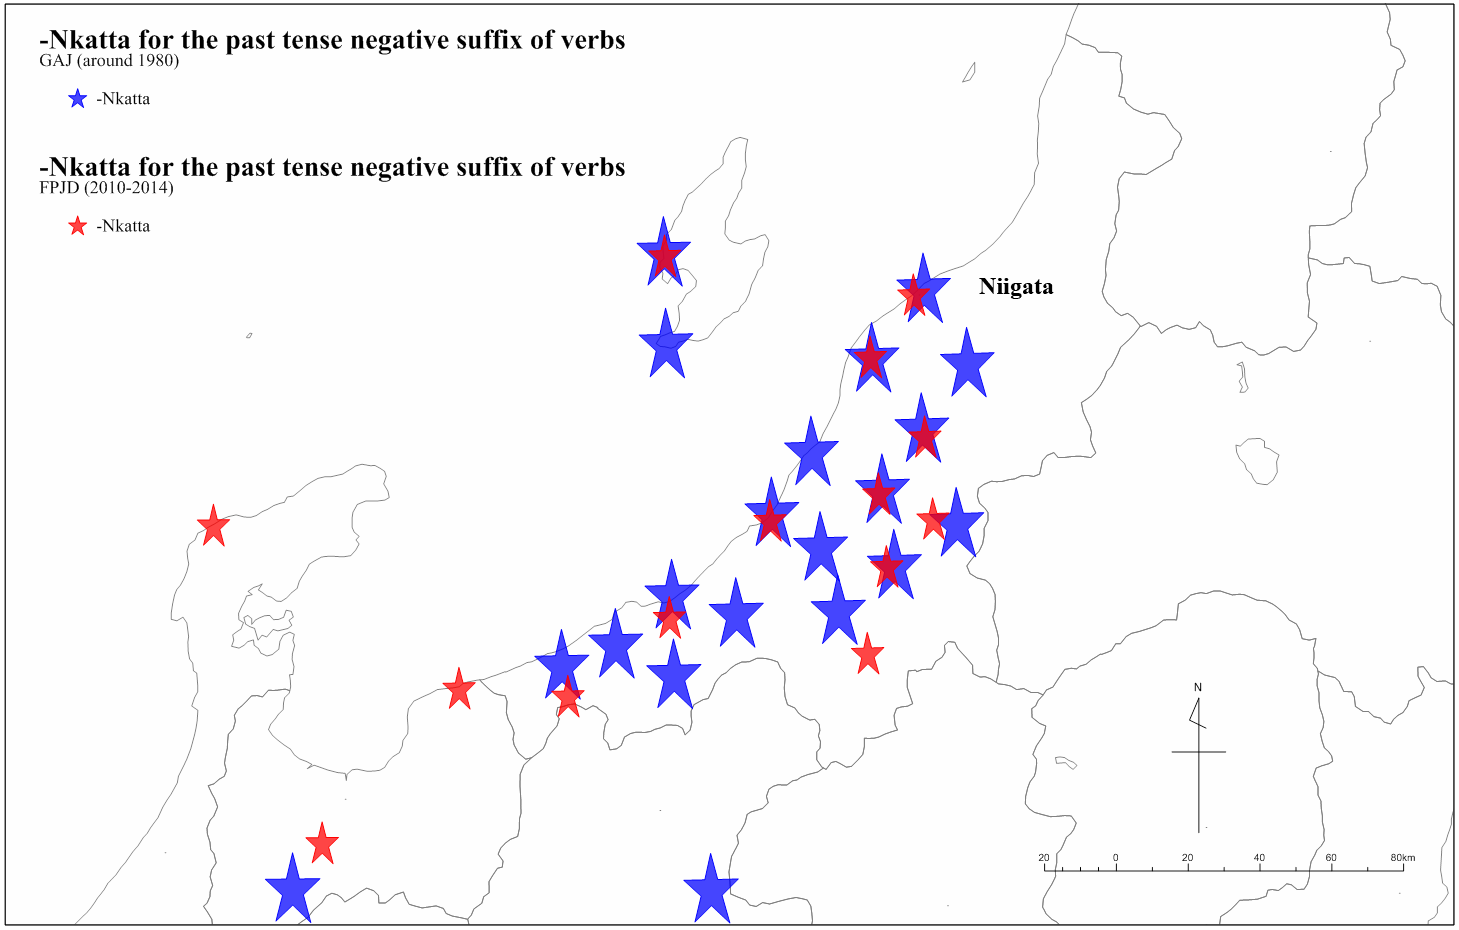
\includegraphics[width=\textwidth]{illustrations/onishi_fig8}
\caption{The distribution of the past-tense negative verb suffix \textit{-Nkatta} in Niigata over a 30-year period.}
\label{fig:8}
\end{figure}

\section{Conclusions}
The examples presented in this paper confirm the hypothesis about how linguistic changes in dialectal distribution spread. A real-time interval comparison shows that new areas of dialectal distributions of linguistic change are formed abruptly and quickly, and not continually or gradually. Rather than expanding from a center in a radial fashion, linguistic changes within dialects appear to start in areas that are not necessarily central, and expand until they fill the area where the people communicate in the relevant dialect. Stability in dialectal distributions is not rare. After the formation of a new distribution area, some dialectal distributions do not change any further.

The reason for this stability can be related to the function of language as a means of communication. Once a linguistic change has started, its use needs to become widespread enough so the language can continue to fulfil this role. This causes new forms to diffuse quickly, but only  to fill the community area. On the other hand, since linguistic changes obstruct smooth communication, they do not continue to easily expand once the area of dialectal distribution is filled.

The examples suggest that the hypothesis is verified. Future work on additional examples aims to further test the hypothesis.

\printbibliography[heading=subbibliography,notkeyword=this]
\end{document}